% !TEX TS-program = pdflatex
% !TEX encoding = UTF-8 Unicode

\documentclass[12pt,addpoints]{exam} % use larger type; default would be 10pt
\usepackage[utf8]{inputenc} % set input encoding (not needed with XeLaTeX)
\usepackage{listings}
\usepackage{amssymb} % for \nmid


%%% Examples of Article customizations
% These packages are optional, depending whether you want the features they provide.
% See the LaTeX Companion or other references for full information.

%%% PAGE DIMENSIONS
\usepackage{geometry} % to change the page dimensions
\geometry{a4paper} % or letterpaper (US) or a5paper or....
% \geometry{margins=2in} % for example, change the margins to 2 inches all round
% \geometry{landscape} % set up the page for landscape
%   read geometry.pdf for detailed page layout information


% \usepackage[parfill]{parskip} % Activate to begin paragraphs with an empty line rather than an indent

%%% PACKAGES
\usepackage{booktabs} % for much better looking tables
\usepackage{array} % for better arrays (eg matrices) in maths
\usepackage{paralist} % very flexible & customisable lists (eg. enumerate/itemize, etc.)
\usepackage{verbatim} % adds environment for commenting out blocks of text & for better verbatim
\usepackage{subfig} % make it possible to include more than one captioned figure/table in a single float
\usepackage{amsthm} % for proof environment
% These packages are all incorporated in the memoir class to one degree or another...
\usepackage{amsfonts} % allows use of mathbb 
\usepackage{amsmath}
\usepackage{multicol}
\usepackage{graphicx} % support the \includegraphics command and options


%%% HEADERS & FOOTERS
%\usepackage{fancyhdr} % This should be set AFTER setting up the page geometry
%\pagestyle{fancy} % options: empty , plain , fancy
%\renewcommand{\headrulewidth}{0pt} % customise the layout...
%\lhead{}\chead{}\rhead{}
%\lfoot{}\cfoot{\thepage}\rfoot{}

%%% SECTION TITLE APPEARANCE
\usepackage{sectsty}
\allsectionsfont{\sffamily\mdseries\upshape} % (See the fntguide.pdf for font help)
% (This matches ConTeXt defaults)

%%% ToC (table of contents) APPEARANCE
\usepackage[nottoc,notlof,notlot]{tocbibind} % Put the bibliography in the ToC
\usepackage[titles,subfigure]{tocloft} % Alter the style of the Table of Contents
\renewcommand{\cftsecfont}{\rmfamily\mdseries\upshape}
\renewcommand{\cftsecpagefont}{\rmfamily\mdseries\upshape} % No bold!
\newcommand{\Dgrad}[1]{\textsf{grad}\,#1\;}
\newcommand{\del}[1] {\mathrm{d}#1\ }
\newcommand{\Q}{\mathbb{Q}}
\newcommand{\F}{\mathbb{F}}
\newcommand{\C}{\mathbb{C}}
\newcommand{\Z}{\mathbb{Z}}
\newcommand{\R}{\mathbb{R}}
\newcommand{\N}{\mathbb{N}}
\newcommand{\PP}{\mathbb{P}}
\newcommand{\arcsec}{\mbox{arcsec}}
\newcommand{\arccsc}{\mbox{arccsc}}
\newcommand{\arccot}{\mbox{arccot}}
\newcommand{\csch}{\mbox{csch}}
\newcommand{\sech}{\mbox{sech}}

%%% NEW ENVIRONMENTS
\newtheorem{theorem}{Theorem}
\newtheorem{definition}[theorem]{Definition}
\newtheorem{example}[theorem]{Example}
\newtheorem{proposition}[theorem]{Proposition}
\newtheorem{corollary}[theorem]{Corollary}
\newtheorem{lemma}[theorem]{Lemma}

%%% END Article customizations

%%% The "real" document content comes below...


\usepackage{color}
\lstset{numbers=left}
\begin{document}

\printanswers

\title{Calculus BC}
\maketitle



\begin{center}
    This exam has \numquestions\ questions for a total of \numpoints\
    points. You have {\bf 4 Hours} to complete this exam.
\end{center}

% this is a 2 hour exam, so each question is for 1 week.
% all sections refer to Thomas and Finney

\section{Statements}
\begin{questions}
    \question[1] State the point-slope equation of a line.
    \begin{solution}
        The point-slope equation of a line through the point $(x_1, y_1)$
        with slope $m$ is $$y - y_1 = m(x - x_1).$$
    \end{solution}

    \question[1] State the slope-intercept equation of a line.
    \begin{solution}
        The slope-intercept equation of a line through with slope $m$
        and $y$-intercept is $$y = mx + b.$$
    \end{solution}

    \question[1] Define the derivative of a function $f$ at a point $x$.
    \begin{solution}
        \begin{definition}
        The derivative of a function $f$ at a point $x$ exists if the
        following limit does, and is equal to this limits value:
        $$f'(x) = \lim_{\Delta h \to 0} \frac{f(x + \Delta x) -
          f(x)}{\Delta x}$$
        \end{definition}
    \end{solution}

    \question[1] State the triangle inequality.
    \begin{solution}
        \begin{theorem}
        For all numbers $a$ and $b$:
        $$|a + b| \le |a| + |b|$$
        \end{theorem}
    \end{solution}

    \question[1] Define the limit of a function $f(x)$ as $c$ approaches
    $t$.
    \begin{solution}%
        \begin{definition} The limite of $f(x)$ as $c$ approaches $t$
        exists and is the number $L$ if given any $\epsilon > 0$ There
        exists $\delta > 0$ such that for all $x$ such that $0 < | x -
        c| < \delta$ implies that $|f(x) - L| < \epsilon$.
        \end{definition}
   
    \end{solution}
    \question[1] State the Sandwich Theorem.
    \begin{solution}

        \begin{theorem} Suppose that $$f(t) \le g(t) \le h(t)$$ for
        all $t \ne c$ in some interval about $c$ and that $f(t)$ and
        $h(t)$ approach the same limit $L$ as $t$ approaches
        $c$. Then $$\lim_{t \to c} g(t) = L$$.
        \end{theorem}
    \end{solution}

    \question[1] State the definition of continuity of a function
    $f(x)$ at a point $x = c$.
    \begin{solution}
        \begin{definition}
        The function $f$ is continuous at a point $x = c$ if
        \begin{enumerate}
        \item $f(c)$ exists
        \item $\lim_{x \to c} f(x)$ exists
        \item $\lim_{x \to c} f(x) = f(c)$.
        \end{enumerate}
        \end{definition}
    \end{solution}

    \question[1] State the intermediate value theorem.
    \begin{solution}   
        \begin{theorem}
            If $f$ is continuous at every point of the interval $[a,
            b]$ and $N$ is any number between $f(a)$ and $f(b)$ then
            there exists $c \in [a, b]$ such that $f(c) = N$.
        \end{theorem}
    \end{solution}

    \question[1] State Rolle's Theorem.
    \begin{solution}
        \begin{theorem}
            Suppose that $y = f(x)$ is continuous at every point of
            the closed interval $[a, b]$ and differentiable at every
            point of its interior $(a, b)$. If 
            $$f(a) = f(b) = 0$$
            then there is at least one number $c$ between $a$ and $b$
            at which $$f'(c) = 0.$$
        \end{theorem}
    \end{solution}

    \question[1] State the Mean Value Theorem
    \begin{solution}
        \begin{theorem}
            If $y = f(x)$ is continuous at every point of the interval
            $[a, b]$ and differentiable in $(a, b)$ then there is at
            least one number $c$ between $a$ and $b$ at which 
            $$\frac{f(b) - f(a)}{b - a} = f'(c).$$
        \end{theorem}
    \end{solution}

    \question[1] State the First Fundamental Theorem of Calculus
    \begin{solution}
        \begin{theorem}
            If $f$ is continuous on $[a, b]$, then
            $$F(x) = \int_a^x f(t)\ dt$$
            is differentiable at every point $x$ in $[a, b]$, and
            $$\frac{dF}{dx} = \frac{d}{dx} \int_a^x f(t)\ dt = f(x).$$
        \end{theorem}
    \end{solution}

    \question[1] State the Second Fundamental Theorem of Calculus
    \begin{solution}
        \begin{theorem}
            If $f$ is continuous at every point of $[a, b]$, and $F$
            is any antiderivative of $f$ on $[a, b]$, then
            $$\int_a^b f(x)\ dx = F(b) - F(a).$$
        \end{theorem}
    \end{solution}

    \question[1] State the definition of the Natural Logarithm
    Function $\ln x$.
    \begin{solution}
        \begin{definition}
            If $x > 0$, then $\ln x = \int_1^x \frac{1}{t}\ dt.$
        \end{definition}
    \end{solution}

    \question[1] State the definition of an improper integral
    $\int_a^b f(x)\ dx$.
    \begin{solution}
        \begin{definition}
            \begin{enumerate}
            \item If $f$ becomes infinite at one or more points of the
                interval of integration or,  
            \item One or both of the limits of integration is
                infinite, or
            \item both (1) and (2) hold.
            \end{enumerate}
        \end{definition}
    \end{solution}
\end{questions}

\section{Multiple Choice}
\begin{questions}       

% Section 1.2
% This is Thomas/Finney 1.2
\question[2] A line $L$ goes through two points: $(1, 2)$ and $(-3,
        4)$. If $L'$ is a line perpendicular to $L$ then the slope of
        $L'$ is
    
    \begin{oneparchoices}
    \choice $-2$
    \choice $2$
    \choice $\frac{1}{2}$
    \CorrectChoice $-\frac{1}{2}$
    \choice nonexistent
    \end{oneparchoices}

% Section 1.6
% This is Thomas/Finney 1.6 Example 6
\question[2] The equation for the tangent line to the curve $y = x^3 +
    3x + 3$ at the point $(0, 3)$ is

    \begin{oneparchoices}
    \CorrectChoice $y = -3x + 3$
    \choice $y = 3x + 3$
    \choice $y = 2x + 3$
    \choice $y = \frac{3}{2}x + 3$
    \choice $y = -2x - 3$
    \end{oneparchoices}

% Section 1.7
% This is 1993 Calculus BC: Section I problem 2
\question[2] If $f(x) = 2x^2 + 1$, then $\lim_{x \to 0} \frac{f(x) -
    f(0)}{x^2}$ is
    
    \begin{oneparchoices}
    \choice $0$
    \choice $1$
    \CorrectChoice $2$
    \choice $4$
    \choice nonexistent
    \end{oneparchoices}

% Section 1.11
% This is 1993 Calculus BC: Section I problem 10
\question[2] Which of the following are continuous at $x = 1$?
    \begin{enumerate}
    \item[I] $\ln x$
    \item[II] $e^{x}$
    \item[III] $\ln(e^{x} - 1)$
    \end{enumerate}

    \begin{oneparchoices}
    \choice I only
    \choice II only
    \choice I and II only
    \choice II and III only
    \CorrectChoice I, II, and III
    \end{oneparchoices}


% Section 1.11
% This is 1993 Calculus BC: Section I problem 44
\question[2] If $f$ is continuous on the interval $[a, b]$, then there
    exists $c$ such that $a < c< b$ and $\int_a^b f(x)dx = $

    \begin{oneparchoices}
    \choice $\frac{f(c)}{b - a}$
    \choice $\frac{f(b) - f(a)}{b - a}$
    \choice $f(b) - f(a)$
    \choice $f'(c)(b - a)$
    \CorrectChoice $f(c)(b - a)$
    \end{oneparchoices}

% Section 1.11
% Thomas/Finney 1.11 example 12
\question[2] Which Theorem can you apply to the function $f(x) = x^3 -
    1$ to conclude that there is a number $1$ less than its cube?
    \begin{oneparchoices}
    \choice The Min-Max Theorem
    \CorrectChoice The Intermediate Value Theorem
    \choice The Mean Value Theorem
    \choice The Sandwich Theorem
    \choice The Limit Combination Theorem.
    \end{oneparchoices}

% Section 2.2
% This is 1993 Calculus BC: Section I problem 21
\question[2] The value of the derivative of $y = \frac{\sqrt[3]{x^2 +
    8}}{\sqrt[4]{2x + 1}}$ at $x = 0$ is

    \begin{oneparchoices}
    \CorrectChoice $-1$
    \choice $-\frac{1}{2}$
    \choice $0$
    \choice $\frac{1}{2}$
    \choice $1$
    \end{oneparchoices}

% Section 2.3
% This is 1993 Calculus BC: Section I problem 17
\question[2] The slope of the tangent line to the graph of $\ln(xy) =
    x$ at the point where $x = 1$ is

    \begin{oneparchoices}
    \CorrectChoice 0
    \choice 1
    \choice $e$
    \choice $e^2$
    \choice $1 - e$
    \end{oneparchoices}

% Section 2.3
% This is 1993 Calculus BC: Section I problem 18
\question[2] If $e^{f(x)} = 1 + x^2$, then $f'(x) = $

    \begin{oneparchoices}
    \choice $\frac{1}{1 + x^2}$
    \CorrectChoice $\frac{2x}{1 + x^2}$
    \choice $2x(1 + x^2)$
    \choice $2x(e^{1 + x^2})$
    \choice $2x\ln(1 + x^2)$
    \end{oneparchoices}

% Section 2.4
% This is Thomas/Finney 2.4.47
\question[2]  The allowable percentage error in measuring the diameter
    $d$ of a sphere if the volume is to be measured correctly to
    within 3\% is

    \begin{oneparchoices}
    \choice within $\pi$\%.
    \choice within 4\%.
    \choice within 3\%.
    \choice within $\frac{4}{3}$\%.
    \CorrectChoice within 1\%.
    \end{oneparchoices}

% Section 2.5
% This is 1993 Calculus BC: Section I problem 4
\question[2] A particle moves along the curve $xy = 10$. If $x = 2$
    and $\frac{dy}{dt} = 3$, what is the value of $\frac{dx}{dt}$?
    
    \begin{oneparchoices}
    \choice $-\frac{5}{2}$
    \CorrectChoice $-\frac{6}{5}$
    \choice $0$
    \choice $\frac{4}{5}$
    \choice $\frac{6}{5}$
    \end{oneparchoices}


% Section 2.5
% This is 1993 Calculus BC: Section I problem 6
\question[2] If $x = t^2 + 1$ and $y = t^3$, then $\frac{d^2y}{dx^2} = $

    \begin{oneparchoices}
    \CorrectChoice $\frac{3}{4t}$
    \choice $\frac{3}{2t}$
    \choice $3t$
    \choice $6t$
    \choice $\frac{3}{2}$.
    \end{oneparchoices}


% Section 2.7
% This is 1993 Calculus BC: Section I problem 12
\question[2] The position of a particle moving along the $x$-axis is
    $x(t) = \sin(2t) - \cos(3t)$ for time $t \ge 0$. What $t = \pi$
    the acceleration of the particle is

    \begin{oneparchoices}
    \choice 9
    \choice $\frac{1}{9}$
    \choice 0
    \choice $-\frac{1}{9}$
    \CorrectChoice $-9$
    \end{oneparchoices}

% Section 2.7
% This is 1993 Calculus BC: Section I problem 15
\question[2] If $f(x) = e^{\tan^2 x}$, then $f'(x) = $

    \begin{oneparchoices}
    \choice $e^{\tan^2 x}$
    \choice $\sec^2 x\ e^{\tan^2 x}$
    \choice $\tan^2 x\ e^{\tan^2 x - 1}$
    \CorrectChoice $2\tan x\ \sec^2 x\ e^{\tan^2 x}$
    \choice $2\tan x\ e^{\tan^2 x}$.
    \end{oneparchoices}

% Section 2.8
% This is 1993 Calculus BC: Section I problem 25
\question[2] Consider the curve in the $xy$-plane represented by $x =
    e^t$ and $y = te^{-t}$ for $t \ge 0$. The slope of the line
    tangent to the curve at the point where $x = 3$ is

    \begin{oneparchoices}
    \choice 20.086
    \choice 0.342
    \choice -0.005
    \CorrectChoice -0.011
    \choice -0.033
    \end{oneparchoices}

% Section 2.9
% This is Thomas/Finney 2.9 Example 2
\question[2] Let $y = x^3 - x$. In Newton's method to find the
    $x$-coordinate of the point where this curve crosses the
    horizontal line $y = 1$ the estimation after 2 iterations is
    approximately
    
    \begin{oneparchoices}
    \CorrectChoice $1.325$
    \choice $0.101$
    \choice $4.450$
    \choice $1.348$
    \choice $0.325$
    \end{oneparchoices}

% Section 3.1
% This is 1993 Calculus BC: Section I problem 22
\question[2] If $f(x) = x^2e^x$, then the graph of $f$ is decreasing
    for all $x$ such that

    \begin{oneparchoices}
    \choice $x < -2$
    \CorrectChoice $-2 < x < 0$
    \choice $x > -2$
    \choice $x < 0$
    \choice $x > 0$
    \end{oneparchoices}

% Section 3.2/3.3
% This is Thomas/Finney 3.3.27
\question[2] Which of the following are true about the graph of $$y
    = \frac{x^2 - 4}{x - 1}$$

    \begin{enumerate}
    \item It has an Asymptote $x = 1$
    \item It is concave up on $(-\infty, 1)$
    \item It has asymptote $y = x + 1$
    \end{enumerate}

    \begin{oneparchoices}
    \choice I Only.
    \choice II Only.
    \choice I and II Only.
    \choice II and II Only.
    \CorrectChoice I, II and III.
    \end{oneparchoices}

% Section 3.4
% This is 1993 Calculus BC: Section I problem 9
\question[2] If $f(x) = 1 + x^{\frac{2}{3}}$, which of the following
    is NOT true?

    \begin{oneparchoices}
    \choice $f$ is continuous for all real numbers.
    \choice $f$ has a minimum at $x = 0$.
    \choice $f$ is increasing for $x > 0$.
    \CorrectChoice $f'(x)$ exists for all $x$.
    \choice $f''(x)$ is negative for all $x > 0$.
    \end{oneparchoices}

% Section 3.4
% This is 1993 Calculus BC: Section I problem 14
\question[2] The {\bf derivative} of $f$ is $x^4(x - 2)(x + 3)$. At
    how many points will the graph of $f$ have a relative maximum?

    \begin{oneparchoices}
    \choice None
    \CorrectChoice One
    \choice Two
    \choice Three
    \choice Four
    \end{oneparchoices}

% Section 3.5
% This is 1993 Calculus BC: Section I problem 36
\question[2] Consider all right circular cylinders for which the sum
    of the height and circumference is 30 centimeters. What is the
    radius of the one with maximum volume?

    \begin{oneparchoices}
    \choice 3 cm
    \choice 10 cm
    \choice 20 cm 
    \choice $\frac{30}{\pi^2}$ cm
    \CorrectChoice $\frac{10}{\pi}$ cm
    \end{oneparchoices}

% Section 3.6
% This is 1993 Calculus BC: Section I problem 34
\question[2] In the figure below, $PQ$ represents a 40-foot ladder
    with end $P$ against a vertical wall and end $Q$ on level
    ground. If the ladder is slipping down the wall, what is the
    distance $RQ$ at the instant when $Q$ is moving along the ground
    $\frac{3}{4}$ as fast as $P$ is moving down the wall?

    \begin{center}
        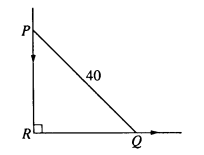
\includegraphics{BC34.png}
    \end{center}

    \begin{oneparchoices}
    \choice $\frac{6}{5}\sqrt{10}$
    \choice $\frac{8}{5}\sqrt{10}$
    \choice $\frac{80}{\sqrt{7}}$
    \choice $24$
    \CorrectChoice $32$
    \end{oneparchoices}

% Section 3.7
% This is 1993 Calculus BC: Section I problem 35
\question[2] If $F$ and $f$ are differentiable functions such that
    $F(x) = \int_0^x f(t)dt$, and $F(a) = -2$ and $F(b) = -2$ where $a
    < b$, which of the following must be true?

    \begin{oneparchoices}
    \CorrectChoice $f(x) = 0$ for some $x$ such that $a < x < b$.
    \choice $f(x) > 0$ for all $x$ such that $a < x < b$.
    \choice $f(x) < 0$ for all $x$ such that $a < x < b$.
    \choice $F(x) \le 0$ for all $x$ such that $a < x < b$.
    \choice $F(x) = 0$ for some $x$ such that $a < x < b$.
    \end{oneparchoices}

% Section 3.7
% These are corollaries 1, 2, and 3 of Thomas/Finney Section 3.7
\question[2] Which of the following are not corollaries of the Mean
    Value Theorem
    
    \begin{enumerate}
    \item $f$ increases when $f' > 0$.
    \item Rolle's theorem
    \item If $F' = 0$ then $F$ is a constant.
    \end{enumerate}

    \begin{oneparchoices}
    \choice I only
    \CorrectChoice II only
    \choice III Only
    \choice I and II only.
    \choice II and III only.    
    \end{oneparchoices}

% Section 3.8
% This is 1993 Calculus BC: Section I problem 24
\question[2] Let $f$ and $g$ be functions that are differentiable for
    all real numbers, with $g(x) \ne 0$ for $x \ne 0$. If $\lim_{x \to
    0} f(x) = \lim_{x \to 0} g(x) = 0$ and $\lim_{x \to
    0} \frac{f'(x)}{g'(x)}$ exists, then $\lim_{x \to
    0} \frac{f(x)}{g(x)}$ is 

    \begin{oneparchoices}
    \choice 0
    \choice $\frac{f'(x)}{g'(x)}$
    \CorrectChoice $\lim_{x \to 0} \frac{f'(x)}{g'(x)}$
    \choice $\frac{f'(x)g(x) - f(x)g'(x)}{(f(x))^2}$
    \choice nonexistent
    \end{oneparchoices}

% Section 3.8
% This is 1993 Calculus BC: Section I problem 42
\question[2] $\lim_{x \to 0} (1 + 2x)^{\csc x} = $

    \begin{oneparchoices}
    \choice $0$
    \choice $1$
    \choice $2$
    \choice $e$
    \CorrectChoice $e^2$
    \end{oneparchoices}

% Section 3.9
% This is Thomas/Finney Section 3.9 Example 3
\question[2] Use the extended mean value theorem to find the error in
    the quadratic approximation of $\sin x$ near $x = 0$ in the
    interval $x \le 0.3$.

    \begin{oneparchoices}
    \CorrectChoice $0.0045$
    \choice $x$
    \choice $0.3$
    \choice $\frac{1}{6}$
    \choice $0.015$
    \end{oneparchoices}

% Section 4.2
% This is Thomas/Finney Example 1
\question[2] Find the curve whose slope at the point $(x, y)$ is
    $3x^2$ if the curve is also required to pass through the point
    $(1, -1)$.

    \begin{oneparchoices}
    \choice $6x - 7$
    \CorrectChoice $x^3 - 2$
    \choice $x^3 + 2$
    \choice $6x + 7$
    \choice $3x^2 - 2$
    \end{oneparchoices}

% Section 4.3
% This is Thomas/Finney Example 5
\question[2] $\int \frac{(z+1)dz}{\sqrt[3]{3z^2 + 6z + 5}}1 = $

    \begin{oneparchoices}
    \choice $\frac{1}{5}(6z + 5)^{\frac{2}{3}} + C$
    \choice $\frac{1}{36}(3z^2 + 6z + 5)^{\frac{1}{3}} + C$
    \choice $\frac{1}{4}(3z^2 + 6z + 5) + C$
    \CorrectChoice $\frac{1}{4}(3z^2 + 6z + 5)^{\frac{2}{3}} + C$
    \choice $\frac{1}{4}(3z^2 + 6z)^{\frac{2}{3}} + C$
    \end{oneparchoices}

% Section 4.4
% This is: Thomas/Finney Example 10
\question[2] $\int \cos^2 x\ dx = $

    \begin{oneparchoices}
    \choice $x + \sin 2x + C$
    \choice $\frac{x}{2} + \frac{\cos 2x}{4} + C$
    \CorrectChoice $\frac{x}{2} + \frac{\sin 2x}{4} + C$
    \choice $\frac{x}{2} + \frac{\sin x}{4} + C$
    \choice  $\frac{x}{2} + \frac{\sin 2x}{2} + C$
    \end{oneparchoices}

% Section 4.5
% This is: 1993 AP Calculus BC Section I Problem 1
\question[2] The area of the region enclosed by the graphs of $y = x^2$
    and $y = x$ is:

    \begin{oneparchoices}
    \CorrectChoice $\frac{1}{6}$
    \choice $\frac{1}{3}$
    \choice $\frac{1}{2}$
    \choice $\frac{5}{6}$
    \choice $1$
    \end{oneparchoices}

% Section 4.5
% This is 1993 Calculus BC: Section I problem 32
\question[2] If $\int_a^b f(x)dx = 5$ and $\int_a^b g(x)dx = -1$ which
    of the following must be true?
    \begin{enumerate}
    \item[I]   $f(x) > g(x)$ for $a \le x \le b$
    \item[II]  $\int_a^b (f(x) + g(x))dx = 4$
    \item[III] $\int_a^b (f(x)g(x))dx = -5$
    \end{enumerate}

    \begin{oneparchoices}
    \choice I only
    \CorrectChoice II only
    \choice III only
    \choice II and III only
    \choice I, II and III
    \end{oneparchoices}

% Section 4.6
% This is Thomas/Finney Review Question 9 in Chapter 4
\question[2] Which of the following are true?
    \begin{enumerate}
    \item[I]   If $\int_a^b f(x)\ dx$ exists, then $f$ is differentiable.
    \item[II]  If $f$ is continuous on $[a, b]$, then $\int_a^b f(x)\
    dx$ exists. 
    \item[III] If $f$ is continuous on $[a, b]$ then $F(x) = \int_a^x
    f(t)\ dt$ is differentiable on $[a, b]$.
    \end{enumerate}

    \begin{oneparchoices}
    \choice I only
    \choice II only
    \choice III only
    \choice II and III only
    \CorrectChoice I, II and III
    \end{oneparchoices}

% Section 4.7
% This is 1993 Calculus BC: Section I problem 33
\question[2] Which of the following is equal to $\int_0^\pi \sin x\ dx$?

    \begin{oneparchoices}
    \choice $\int_{-\frac{\pi}{2}}^\frac{\pi}{2} \cos x\ dx$
    \CorrectChoice $\int_0^\pi \cos x\ dx$
    \choice $\int_{-\pi}^0 \sin x\ dx$
    \choice $\int_{-\frac{\pi}{2}}^\frac{\pi}{2} \sin x\ dx$
    \choice $\int_\pi^{2\pi} \sin x\ dx$
    \end{oneparchoices}

% Section 4.7
% This is 1993 Calculus BC: Section I problem 41
\question[2] Let $f(x) = \int_{-2}^{x^2 - 3x} e^{t^2}\ dt.$ At what
    value of $x$ is $f(x)$ a minimum?

    \begin{oneparchoices}
    \choice For no value of $x$
    \choice $\frac{1}{2}$
    \CorrectChoice $\frac{3}{2}$
    \choice $2$
    \choice $3$
    \end{oneparchoices}

% Section 4.9
% This is: Thomas/Finney Examples 1 and 2
\question[2] Using the trapezoidal rule with $n = 4$ to estimate
             $$\int_1^2 x^2\ dx$$ gives (using the error formula):

    \begin{oneparchoices}
    \choice Estimate of $\frac{7}{3}$ with upper bound for error of $\frac{1}{48}$.
    \choice Estimate of $\frac{75}{16}$ with upper bound for error of $\frac{1}{48}$.
    \choice Estimate of $\frac{7}{3}$ with upper bound for error of $\frac{1}{96}$.
    \choice Estimate of $2.34375$ with upper bound for error of $\frac{1}{192}$.
    \CorrectChoice Estimate of $2.34375$ with upper bound for error of $\frac{1}{96}$.
    \end{oneparchoices}

% Section 4.9
% This is 1993 Calculus BC: Section I problem 40
\question[2] Let $R$ be the region in the first quandrant enclosed by
    the $x$-acis and the graph of $y = \ln(1 + 2x - x^2)$. If
    Simpson's Rule with 2 subintervals is used to approximate the area
    of $R$, the approximation is

    \begin{oneparchoices}
    \choice $0.462$
    \choice $0.693$
    \CorrectChoice $0.924$
    \choice $0.986$
    \choice $1.850$
    \end{oneparchoices}

% Section 5.1
% This is 1993 Calculus BC: Section I problem 20
\question[2] A particle moves along the $x$-axis so that at any time
    $t \ge 0$ the acceleration of the particle is $a(t) = e^{-2t}$. If
    at $t = 0$ the velocity of the particle is $\frac{5}{2}$ and its
    position is $\frac{17}{4}$, then its position at any time $t > 0$
    is $x(t) = $

    \begin{oneparchoices}
    \choice $-\frac{e^{-2t}}{2} + 3$
    \choice $\frac{e^{-2t}}{4} + 4$
    \choice $4e^{-2t} + \frac{9}{2}t + \frac{1}{4}$
    \choice $\frac{e^{-2t}}{2} + 3t + \frac{15}{4}$
    \CorrectChoice $\frac{e^{-2t}}{4} + 3t + 4$
    \end{oneparchoices}

% Section 5.3
% This is 1993 Calculus BC: Section I problem 30
\question[2] What is the volume of the solid generated by rotating
    about the $x$-axis the region enclosed by the curve $y = \sec x$
    and the lines $x = 0$, $y = 0$, and $x = \frac{pi}{3}$?

    \begin{oneparchoices}
    \choice $\frac{\pi}{3}$
    \choice $\pi$
    \CorrectChoice $\pi\sqrt{3}$
    \choice $\frac{8\pi}{3}$
    \choice $\pi\ln(\frac{1}{2} + \sqrt{3})$
    \end{oneparchoices}

% Section 5.4 (Cyclindrical Shells)
% This is 1993 Calculus BC: Section I problem 19
\question[2] The region bounded by the $x$-axis and $y = kx - x^2$
    between $x = 0$ and $x = k$ is rotated about the {\bf $y$-axis} to
    form a solid whose volume is 10 cubic units. Of the following,
    which best approximates $k$?

    \begin{oneparchoices}
    \choice $1.51$
    \CorrectChoice $2.09$
    \choice $2.49$
    \choice $4.18$
    \choice $4.77$
    \end{oneparchoices}

% Section 5.5
% This is 1993 Calculus BC: Section I problem 23
\question[2] The length of the curve determined by the equations $x =
    t^2$ and $y = t$ from $t = 0$ to $t = 4$ is

    \begin{oneparchoices}
    \choice $\int_0^4 \sqrt{4t + 1}\ dt$
    \choice $2\int_0^4\sqrt{t^2 + 1}\ dt$
    \choice $\int_0^4\sqrt{2t^2 + 1}\ dt$
    \CorrectChoice $\int_0^4\sqrt{4t^2 + 1}\ dt$
    \choice $2\pi\int_0^4\sqrt{4t^2 + 1}\ dt$
    \end{oneparchoices}

% Section 5.7
% This is 1993 Calculus BC: Section I problem 39
\question[2] If $\frac{dy}{dx} = \frac{1}{x},$ then the average rate
    of change of $y$ with respect to $x$ on the closed interval $[1,
    4]$ is

    \begin{oneparchoices}
    \choice $-\frac{1}{4}$
    \choice $\frac{1}{2}\ln 2$
    \CorrectChoice $\frac{2}{3}\ln 2$
    \choice $\frac{2}{5}$
    \choice $2$
    \end{oneparchoices}

% Section 6.3
% This is 1993 Calculus BC: Section I problem 26
\question[2] If $y = \arctan(e^{2x})$, then $\frac{dy}{dx} =$

    \begin{oneparchoices}
    \choice $\frac{2e^{2x}}{\sqrt{1 - e^{4x}}}$
    \CorrectChoice $\frac{2e^{2x}}{1 + e^{4x}}$
    \choice $\frac{e^{2x}}{1 + e^{4x}}$
    \choice $\frac{1}{\sqrt{1 - e^{4x}}}$
    \choice $\frac{1}{1 + e^{4x}}$
    \end{oneparchoices}

% Section 6.3
% This is: Thomas/Finney Example 3
\question[2] $\int \frac{x^2 dx}{\sqrt{1 - x^6}} = $

    \begin{oneparchoices}
    \CorrectChoice $\frac{1}{3}\arcsin(x^3) + C$
    \choice $\frac{1}{3}\arccos(x^3) + C$ 
    \choice $6\arcsin(x) + C$
    \choice $\arcsin(x^3) + C$
    \choice $3\arcsin(x^3) + C$
    \end{oneparchoices}

% Section 6.3
% This is: Thomas/Finney Example 2b
\question[2]
    $\int_{\frac{2}{\sqrt{3}}}^{\sqrt{2}} \frac{dx}{x\sqrt{x^2 - 1}} = $

    \begin{oneparchoices}
    \choice $0$
    \choice $\frac{1 - \sqrt{3}}{2}$
    \choice $1 - \sqrt{3}$
    \choice $\frac{\pi}{3}$
    \CorrectChoice $\frac{\pi}{12}$
    \end{oneparchoices}

% Section 6.4
% This is 1993 Calculus BC: Section I problem 37
\question[2] If $f(x) = \left\{ \begin{array}{lr} x & \mbox{for } x \le
    1 \\ \frac{1}{x} & \mbox{for } x > 1, \end{array} \right.$ then $\int_0^e
    f(x)dx = $

    \begin{oneparchoices}
    \choice $0$
    \CorrectChoice $\frac{3}{2}$
    \choice $2$
    \choice $e$
    \choice $e + \frac{1}{2}$
    \end{oneparchoices}

% Section 6.4
% This is: Thomas/Finney problem 19
\question[2]  If $y = x[\sin (\ln x) + \cos (\ln x)]$, then
    $\frac{dy}{dx} = $

    \begin{oneparchoices}
    \choice $\cos (\ln x)$
    \choice $1$
    \CorrectChoice $2 \cos(\ln x)$
    \choice $\cos (x)$
    \choice $x$
    \end{oneparchoices}

% Section 6.6
% This is 1993 Calculus BC: Section I problem 8
\question[2] If $f(x) = \ln(e^{2x})$, then $f'(x) = $

    \begin{oneparchoices}
    \choice $1$
    \CorrectChoice $2$
    \choice $2x$
    \choice $e^{-2x}$
    \choice $2e^{-2x}$
    \end{oneparchoices}

% Section 6.6
% This is 1993 Calculus BC: Section I problem 7
\question[2] $\int_0^1 x^3e^{x^4}\ dx =$

    \begin{oneparchoices}
    \CorrectChoice $\frac{1}{4}(e - 1)$
    \choice $\frac{1}{4}e$
    \choice $e - 1$
    \choice $e$
    \choice $4(e - 1)$
    \end{oneparchoices}

% Section 6.9
% This is 1993 Calculus BC: Section I problem 38
\question[2] During a certain epidemic, the number of people that are
    infected at any time increases at a rate proportional to the
    number of people that are infected at that time. If 1,000 people
    are infected when the epidemic is first discovered, and 1,200 are
    infected 7 days later, how many people are infected 12 days after
    the epidemic is first discovered?

    \begin{oneparchoices}
    \choice 343
    \choice 1,343
    \CorrectChoice 1,367
    \choice 1,400
    \choice 2,057
    \end{oneparchoices}

% Section 
% This is 1993 Calculus BC: Section I problem 11
\question[2] $\int_6^\infty \frac{-2x}{\sqrt[3]{9 - x^2}}\ dx$ is

    \begin{oneparchoices}
    \choice $7^\frac{2}{3}$
    \choice $\frac{3}{2}(7^\frac{2}{3})$
    \choice $9^\frac{2}{3} + 7^\frac{2}{3}$
    \choice $\frac{3}{2}(9^\frac{2}{3} + 7^\frac{2}{3})$
    \CorrectChoice nonexistent
    \end{oneparchoices}


% Section 7.2
% This is 1993 Calculus BC: Section I problem 29
\question[2] $\int x\sec^2 x\ dx = $

    \begin{oneparchoices}
    \choice $x\tan x + C$
    \choice $\frac{x^2}{2}\tan x + C$
    \choice $\sec^2 x + 2\sec^2 x \tan x + C$
    \choice $x\tan x - \ln |\cos x| + C$
    \CorrectChoice $x\tan x + \ln |\cos x| + C$
    \end{oneparchoices}

% Section 7.2
% This is: Thomas/Finney Example 5
\question[2] $\int e^{2x}\cos 3x\ dx = $

    \begin{oneparchoices}
    \CorrectChoice $\frac{3e^{2x} \sin 3x + 2e^{2x} \cos 3x}{13} + C$.
    \choice $\sin 3x - \frac{1}{3} \cos 3x + C$.
    \choice $\frac{e^{2x} \sin 3x + e^{2x} \cos 3x}{13} + C$.
    \choice $\frac{5e^{2x}}{13} + C$.
    \choice $1$
    \end{oneparchoices}

% Section 7.3
% This is: Thomas/Finney Example 4
\question[2] $\int \tan^4 x\ dx = $

    \begin{oneparchoices}
    \choice $\frac{1}{3} \tan^3 x + C$
    \choice $\frac{1}{5} \tan^5 x + C$
    \choice $\frac{1}{5} \tan^5 x \cdot \sec x + C$
    \choice $\frac{1}{3} \tan^3 x - \tan x + \frac{1}{5}x^5 + C$
    \CorrectChoice $\frac{1}{3} \tan^3 x - \tan x + x + C$
    \end{oneparchoices}

% Section 7.3
% This is: Thomas/Finney Example 1
\question[2] $\int \sin^3 x\ dx = $

    \begin{oneparchoices}
    \choice $\frac{\sin^4}{4} + C$
    \CorrectChoice $\frac{\cos^3 x}{3} - \cos x + C$
    \choice $\cos^3 x - \cos x + C$
    \choice $\cos^2 x + C$
    \choice $\frac{\sin^3 x}{3} - \sin x + C$
    \end{oneparchoices}

% Section 7.3
% This is: Thomas/Finney Example 5
\question[2] $\int \sin 3x \cos 5x\ dx = $

    \begin{oneparchoices}
    \choice $-\frac{\cos 8x}{8} + \frac{\cos 2x}{2} + C$
    \choice $-\frac{\cos 8x}{16} + \frac{\sin 2x}{4} + C$
    \choice $-\frac{\cos 10x}{2} + \frac{\cos 6x}{2} + C$
    \CorrectChoice $-\frac{\cos 8x}{16} + \frac{\cos 2x}{4} + C$
    \choice $-\frac{\cos 10x}{16} + \frac{\cos 6x}{4} + C$
    \end{oneparchoices}

% Section 7.4
% This is: Thomas/Finney 35
\question[2] The area between the $x$-axis and the curve $y = \sqrt{1
    + \cos 4x}$, $0 \le x \le \pi$.

    \begin{oneparchoices}
    \choice $\sqrt{2}/2$
    \choice $\sqrt{2}$
    \CorrectChoice $2\sqrt{2}$
    \choice $0$
    \choice $1$
    \end{oneparchoices}

% Section 7.5
% This is: Thomas/Finney 3
\question[2] $\int_{-2}^2 \frac{dx}{4 + x^2} = $

    \begin{oneparchoices}
    \CorrectChoice $\pi/4$
    \choice $0$
    \choice $1$
    \choice $\pi$
    \choice $e$
    \end{oneparchoices}

% Section 7.5
% This is: Thomas/Finney 5
\question[2] $\int_0^{1/2\sqrt{2}} \frac{2\ dx}{\sqrt{1 - 4x^2}} = $

    \begin{oneparchoices}
    \choice $\pi/2$
    \CorrectChoice $\pi/4$
    \choice $\pi$
    \choice $0$
    \choice $e$
    \end{oneparchoices}

% Section 7.5
% This is: Thomas/Finney 11
\question[2] $\int \frac{3\ dz}{\sqrt{9z^2 - 1}} = $ 

    \begin{oneparchoices}
    \choice $\ln|3z + \sqrt{9z^2 + 1}| + C$
    \choice $|3z + \sqrt{9z^2 - 1}| + C$
    \CorrectChoice $\ln|3z + \sqrt{9z^2 - 1}| + C$
    \choice $C$
    \choice $\ln|\tan z| + C$
    \end{oneparchoices}

% Section 7.6
% This is: Thomas/Finney Example 4
\question[2] $\int \frac{dx}{\sqrt{2x - x^2}} = $

    \begin{oneparchoices}
    \choice  $x + C$
    \choice  $\arctan(x - 1) + C$
    \choice  $\arccos(x - 1) + C$
    \CorrectChoice $\arcsin(x - 1) + C$
    \choice  $\arcsin(x + 1) + C$
    \end{oneparchoices}

% Section 7.7
% This is: 1988 AP Calculus BC: Section I,  #17
\question[2] $\int_2^3 \frac{dx}{(x-1)(x+2)} = $

    \begin{oneparchoices}
    \choice  $-\frac{33}{20}$
    \choice  $-\frac{9}{20}$
    \choice  $\ln(\frac{5}{2})$
    \CorrectChoice $\ln(\frac{8}{5})$
    \choice $\ln(\frac{2}{5})$
    \end{oneparchoices}

% Section 7.8
% This is: 1997 AP Calculus BC: Section I, Part A #11
\question[2] $\int_1^\infty \frac{x}{(1+x^2)^2} dx = $

    \begin{oneparchoices}
    \choice  $-\frac{1}{2}$
    \choice  $-\frac{1}{4}$
    \CorrectChoice  $\frac{1}{4}$
    \choice $\frac{1}{2}$
    \choice $divergent$
    \end{oneparchoices}

% Section 7.8
% This is: 1973 AP Calculus BC: Section I,  #36
\question[2] $\int_0^1 \frac{x+1}{x^2 + 2x - 3}\ dx = $

    \begin{oneparchoices}
    \choice $-\ln \sqrt{3}$
    \choice $-\frac{\ln \sqrt{3}}{2}$ 
    \choice $\frac{1 - \ln \sqrt{3}}{2}$ 
    \choice $\ln \sqrt{3}$ 
    \CorrectChoice divergent 
    \end{oneparchoices}

% 745 - 514 + 1136 - 1081 = 286
% 286/19 = 15

% Section 8.1 - 8.3
% This is: Thomas/Finney Example 4
\question[2] A parabola with vertex $(-2, 1)$ and focus $(1, 1)$ is

    \begin{oneparchoices}
    \choice $y^2 + 2y - 12x + 24 = 0$
    \choice $x^2 + 6x + 1 = 0$
    \CorrectChoice $y^2 - 2y - 12x - 23 = 0$
    \choice $x^2 + y + 12x + 24 = 0$
    \choice $x^2 + 2y - 12x = 0$
    \end{oneparchoices}

Should the above be 8.4 question about the main eccentricity equation?

% Section 8.4 - 8.5


% 8.6 - 8.9
% 9.1 - 9.4
% 10.1 - 10.4
% 11.1 - 11.2
% 11.3 - 11.4
% 11.5 
% 11.6 - 11.7
% 11.8 - 11.10
% 12.1 - 12.3
% 12.4 
% 12.5 - 12.6
% 20.1 - 20.3
% 20.4 - 20.5
% 20.6 - 20.9

% Section 10.2
% This is 1993 Calculus BC: Section I problem 5
\question[2] Which of the following represents the graph of the polar
    curve $r = 2\sec \theta$?

    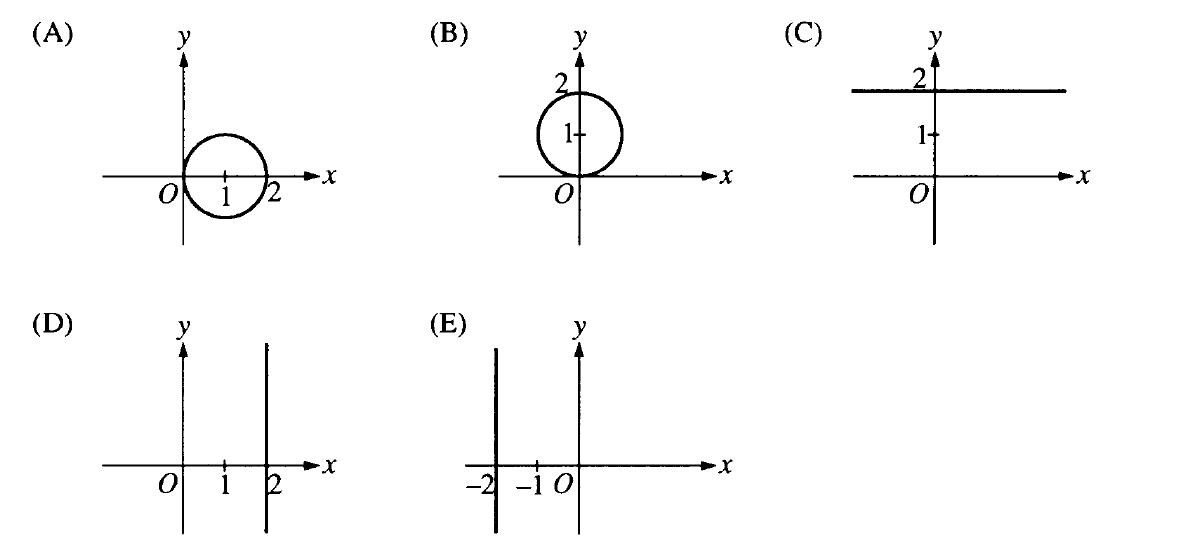
\includegraphics[scale=0.7]{BC5.png}    

% Section 11.2
% This is 1993 Calculus BC: Section I problem 31
\question[2] If $s_n =
(\frac{(5+n)^{100}}{6{n+1}})(\frac{5^n}{(4+n)^{100}})$, to what number
does the sequence $\{s_n\}$ converge?

    \begin{oneparchoices}
    \CorrectChoice $\frac{1}{5}$
    \choice $1$
    \choice $\frac{5}{4}$
    \choice $(\frac{5}{4})^{100}$
    \choice The sequence does not converge.
    \end{oneparchoices}

% Section 11.4 (p-series, geometric, alternating harmonic)
% This is 1993 Calculus BC: Section I problem 16
\question[2] Which of the following series diverge?
            
    \begin{enumerate}
    \item[I] $\sum_{k = 3}^\infty \frac{2}{k^2 + 1}$
    \item[II] $\sum_{k = 1}^\infty (\frac{6}{7})^k$
    \item[III] $\sum_{k = 2}^\infty \frac{(-1)^k}{k}$
    \end{enumerate}

    \begin{oneparchoices}
    \CorrectChoice None
    \choice II only
    \choice III only
    \choice I and III
    \choice II and III
    \end{oneparchoices} 

% Section 11.4 (Geometric Series)
% This is 1993 Calculus BC: Section I problem 45
\question[2] If $f(x) = \sum_{k = 1}^\infty (\sin^2 x)^k$, then $f(1)$ is

    \begin{oneparchoices}
    \choice $0.369$
    \choice $0.585$
    \choice $2.400$
    \CorrectChoice $2.426$
    \choice $3.426$
    \end{oneparchoices}

% Section 12.2
% This is 1993 Calculus BC: Section I problem 43
\question[2] The coefficient of $x^6$ in the Taylor series expansion
    about $x = 0$ for $f(x) = \sin (x^2)$ is

    \begin{oneparchoices}
    \CorrectChoice $-\frac{1}{6}$
    \choice $0$
    \choice $\frac{1}{120}$
    \choice $\frac{1}{6}$
    \choice $1$
    \end{oneparchoices}

% Section 12.5
% This is 1993 Calculus BC: Section I problem 27
\question[2] The interval of convergence of $\sum_{n =
    0}^\infty \frac{ (x-1)^n }{3^n}$ is

    \begin{oneparchoices}
    \choice $-3 < x \le 3$
    \choice $-3 le x \le 3$
    \CorrectChoice $-2 < x < 4$
    \choice $-2 \le x < 4$
    \choice $0 \le x \le 2$
    \end{oneparchoices}

% Section 13.2
% This is 1993 Calculus BC: Section I problem 28
\question[2] If a particle moves in the $xy$-plane so that at time $t
    > 0$ its position vector is $(\ln(t^2 + 2t), 2t^2)$ then at time
      $t = 2$ its velocity vector is

    \begin{oneparchoices}
    \CorrectChoice $(\frac{3}{4}, 8)$
    \choice $(\frac{3}{4}, 4)$
    \choice $(\frac{1}{8}, 8)$
    \choice $(\frac{1}{8}, 4)$
    \choice $(-\frac{5}{16}, 4)$
    \end{oneparchoices}

% Section 20.2
% This is 1993 Calculus BC: Section I problem 13
\question[2] If $\frac{dy}{dx} = x^2y$, then $y$ could be

    \begin{oneparchoices}
    \choice $3\ln(\frac{x}{3})$
    \choice $e^\frac{x^3}{3} + 7$
    \CorrectChoice $2e^\frac{x^3}{3}$
    \choice $3e^{2x}$
    \choice $\frac{x^3}{3} + 1$
    \end{oneparchoices}
\end{questions}

\section{Free Response}
\begin{questions}

% Thomas/Finney 1.7 Example 7
\question[10] Find $\frac{dy}{dx}$ if $y = \frac{1}{x}$ using the
    definition of the derivative. You may use any results on limits
    you wish.

    \begin{solution}
        Note that:
        $$\frac{ f(x+h) - f(x) }{ h } = \frac{ \frac{1}{x+h}
          - \frac{1}{x} }{h}$$
        $$= \frac{1}{h} \cdot \frac{x - (x + h)}{x(x+h)}$$
        $$= \frac{1}{h} \cdot \frac{-h}{x(x+h)} = \frac{-1}{x(x+h)}$$
        Thus,
        $$\frac{dy}{dx} = \lim_{h \to 0} \frac{f(x+h) - f(x)}{h} $$
        $$ = \lim_{h \to 0} \frac{-1}{x(x+h)} = \frac{-1}{x(x+0)} $$
        $$ = -\frac{1}{x^2}.$$
    \end{solution}

% Thomas/Finney 1.11 Theorem 5
\question[10] Prove the following:
              \begin{theorem}
                  A function is continuous at every point at which it
                  has a derivative. That is, if $y = f(x)$ has a
                  derivative $f'(c)$ at $x = c$, then $f$ is
                  continuous at $c$.
              \end{theorem}

    \begin{solution}
        We are given that $f(c)$ exists therefore we need to show that
        $\lim_{x \to c} f(c)$ exists and is equal to $f(c)$.

        $$\lim_{x \to c} (f(x) - f(c)) = \lim_{x \to c} 
            [(x-c)\frac{f(x) - f(c)}{x - c}$$
        $$= 0 \cdot f'(c) = 0$$
    \end{solution}

% 1995 Calculus BC Section II problem 1
%\question (\totalpoints\ points) Two particles move in the
%    $xy$-plane. For time $t \ge 0$, the position of particle $A$ is
%    given by $x = t - 2$ and $y = (t - 2)^2$, and the position of
%    particle $B$ is given by $x = \frac{3t}{2} - 4$ and $y
%    = \frac{3t}{2} - 2.$

%    \begin{parts}
%    \part[3] Find the velocity vector for each particle at time $t =
%    3$.
%    \begin{solution}
%        $$V_A = (1, 2t - 4)$$
%        $$V_A(3) = (1, 2)$$
%        $$V_B = (\frac{3}{2}, \frac{3}{2})$$
%        $$V_B(3) = (\frac{3}{2}, \frac{3}{2})$$
%    \end{solution}
%    \part[3] Setup an integral expression that gives the distance
%    traveled by particle $A$ from $t = 0$ to $t = 3$. Do not evaluate.
%    \begin{solution}
%        $$\int_0^3 \sqrt{1^2 + (2t - 4)^2}\ dt$$
%    \end{solution}
%    \part[5] Determine the exact time at which the particles collide;
%    taht is, when the particles are at the same point at the same
%    time. Justify your answer.
%    \begin{solution}
%        Set $t -2 = \frac{3t}{2} - 4$ and solving gives $t = 4.$. Thus
%        when $t = 4$ the $y$-coordinates for $A$ and $B$ are
%        equal. Particles collide at $(2, 4)$ when $t = 4$.
%    \end{solution}
%    \part[4] In the part of the plane given by $[-7, 7] \times [-5,
%    5]$ sketch the paths of the particles $A$ and $B$ from $t = 0$
%    until they collide. Indicate the direction of each particle along
%    its path.
%    \begin{solution}
%        \begin{center}
%            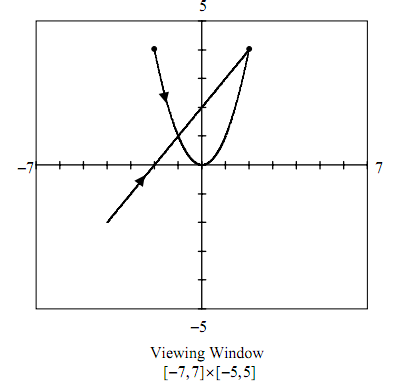
\includegraphics{BC46.png}
%        \end{center}
%    \end{solution}
%    \end{parts}

% Derivation from Section 7.3 of Thomas/Finney
\question[10] Compute $\int \sec x\ dx$.
\begin{solution}
    $$\int \sec x\ dx = \int \frac{1}{\cos x}dx$$
    $$ = \int \frac{\cos x}{\cos^2 x}dx$$
    $$ = \int \frac{\cos x}{1 - \sin^2 x}dx$$
    $$ = \int \frac{\cos x}{(1 - \sin x)(1 + \sin x)} dx$$
    $$ = \frac{1}{2}\int \frac{\cos x}{1 - \sin x} + \frac{\cos x}{1
    + \sin x}\ dx$$
    $$ = \frac{1}{2}[-\ln|1 - \sin x| + \ln|1 + \sin x|] + C$$
    $$ = \frac{1}{2}\ln |\frac{1 + \sin x}{1 - \sin x}| + C$$
    $$ = \frac{1}{2}\ln |\frac{1 + \sin x}{1 - \sin x} \cdot \frac{1 + \sin x}{1 + \sin x}| + C$$
    $$ = \frac{1}{2}\ln |\frac{(1 + \sin x)^2}{1 - \sin^2 x}| + C$$
    $$ = \frac{1}{2}\ln |\frac{(1 + \sin x)^2}{\cos^2 x}| + C$$
    $$ = \ln |\frac{1 + \sin }{\cos x}| + C$$
    $$ = \ln |\sec x + \tan x| + C$$
\end{solution}

% 1995 Calculus BC Section II problem 2
%\question (\totalpoints\ points) The shaded regions $R_1$ and $R_2$
%    shown below are enclosed by the graphs of $f(x) = x^2$ and $g(x) = 2^x$.
%     \begin{center}
%         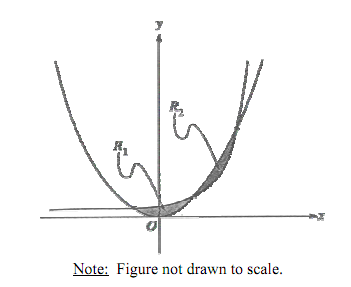
\includegraphics{BCII-2.png}
%     \end{center}

%     \begin{parts}
%     \part[5] Find the $x$- and $y$-coordinates of the three points of
%     intersection of the graphs of $f$ and $g$.
%     \begin{solution}
%         $(2, 4), (4, 16), (-0.767, 0.588)$.
%     \end{solution}
%     \part[5] Without using absolute value, set up an
%     expression involving one or more integrals that gives the total
%     area enclosed by the graphs of $f$ and $g$. Do not evaluate.
%     \begin{solution}
%         $\int_{-0.767}^2 (2^x - x^2)dx + \int_2^4 (x^2 - 2^x)dx$
%     \end{solution}
%     \part[5] Without using absolute value, set up an expression
%     involving one or more integrals that gives the volume of the
%     solid generated by revolving the region $R_1$ about the line $y =
%     5$. Do not evaluate.
%     \begin{solution}
%         $\pi \int_{-0.767}^2 ( (5 - x^2)^2 - (5 - 2^x)^2)dx$
%     \end{solution}
%     \end{parts}

% 1995 Calculus BC Section II problem 4
\question (\totalpoints\ points) Let $f$ be a function that has a
         derivatives of all ordere for all real numbers. Assume $f(1)
         = 3$, $f'(1) = -2$, $f''(2) = 2$, and $f'''(1) = 4$.
      \begin{parts}
      \part[5] Write the second-degree Taylor polynomial for $f$ about
         $x = 1$ and use it to approximate $f(0.7)$.
      \begin{solution}
          $$T_2(x) = 3 + (-2)(x - 1) + \frac{2}{2}(x - 1)^2$$
          $$f(0.7) \approx 3 + 0.6 + 0.09 = 3.69$$
      \end{solution}
      \part[5] Write the third-degree Taylor polynomial for $f$ about
         $x = 1$ and use it to approximate $f(1.2)$.
      \begin{solution}
          $$T_3(x) = 3 - 2(x - 1) + (x - 1)^2 + \frac{4}{6}(x - 1)^3$$
          $$f(1.2) \approx 3 - 0.4 + 0.04 + \frac{2}{3}(0.008) = 2.645$$
      \end{solution}
      \part[5] Write the second-degree Taylor polynomial for $f'$, the
         derivative of $f$ about $x = 1$ and use it to approximate
         $f'(1.2)$.        
      \begin{solution}
          $$T'_3(x) = -2 + 2(x - 1) + 2(x - 1)^2$$
          $$f'(1.2) \approx -2 + 0.4 + 0.08 = -1.52$$
      \end{solution}
      \end{parts}

% 1995 Calculus BC Section II problem 6
\question (\totalpoints\ points) Let $f$ be a function whose domain is
          the closed interval $[0, 5]$. The graph of $f$ is shown
          below.
          
          \begin{center}
              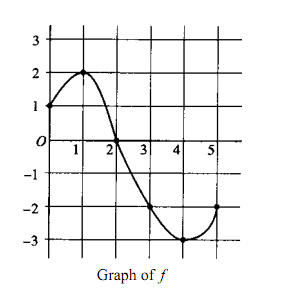
\includegraphics{BCII-6.png}
          \end{center}

          Let $h(x) = \int_0^{\frac{x}{2} + 3} f(t)\ dt$.

          \begin{parts}
          \part[5] Find the domain of $h$.
              \begin{solution}
                  $$0 \le \frac{x}{2} + 3 \le 5$$
                  $$-6 \le x \le 4$$
              \end{solution}
          \part[5] Find $h'(2)$.
              \begin{solution}
                  $$h'(x) = f(\frac{x}{2} + 3) \cdot \frac{1}{2}$$
                  $$h'(2) = f(4) \cdot \frac{1}{2} = - \frac{3}{2}$$
              \end{solution}
          \part[5] At what $x$ is $h(x)$ a minimum? Show the analysis
              that leads to your conclusion.
              \begin{solution}
                  $h'$ is positive, then negative, so minimum is at an
                  endpoint.
                  $$h(-6) = \int_0^0 f(t) dt = 0$$
                  $$h(4) = \int_0^5 f(t) dt < 0$$
                  since the area below the axis is greater than the
                  area above the axis therefore minimum at $x = 4$.
              \end{solution}
          \end{parts}
\end{questions}

\end{document}
